\documentclass{beamer}
\mode<presentation>
{
  	\usetheme{Copenhagen}
	%\usetheme{CambridgeUS}
  	\usecolortheme{whale}
}
\usepackage{hyperref}
\usepackage{psfrag}
\usepackage{color}
\usepackage[english]{babel}
\usepackage[latin1]{inputenc}
\usepackage{times}
\usepackage[T1]{fontenc}
\usepackage{amssymb}
\usepackage{multirow}
\setbeamercovered{dynamic}
%---------------------------------------------------------------------------------------------------------------------------%
%-------------------------------------------------------Title Page----------------------------------------------------------%
%---------------------------------------------------------------------------------------------------------------------------%
\title{Level Crossing Analog to Digital Converters}
\author[Janamani Chandram Ayyangalam]{Janamani C. Ayyangalam \\  08407604 }
\institute[IIT Bombay]{Under the Guidance of \\ \vspace{3 mm} \begin{large} Prof. A. N. Chandorkar \end{large} }
\date[\today]{\today}
\begin{document}
\begin{frame}
\titlepage
\end{frame}
%---------------------------------------------------------------------------------------------------------------------------%
%---------------------------------------------------------Outline-----------------------------------------------------------%
%---------------------------------------------------------------------------------------------------------------------------%
\begin{frame}
	\frametitle{Outline} 
	\begin{itemize} 
		\item{ Motivation }\\
		\item{ Theory of level cross sampling scheme }\\
		\item{ Reported level crossing ADC architectures }\\ 
			\begin{itemize} \footnotesize
				\item{ Level crossing asynchronous ADC }
				\item{ Signal dependent variable resolution ADC }
				\item{ Adaptive asynchronous ADC }
			\end{itemize}
		\item{ Proposed level crossing ADC architectures }
			\begin{itemize} \footnotesize
				\item{ Architecture for high activity signals }
				\item{ Architecture for low activity signals }
			\end{itemize}
		\item{ Conclusion \& Future work }\\
		\item{ References }		
        \end{itemize}
\end{frame}
%%---------------------------------------------------------------------------------------------------------------------------%
%%--------------------------------------------------------Motivation---------------------------------------------------------%
%%---------------------------------------------------------------------------------------------------------------------------%
%\subsection*{Motivation}
%\begin{frame}
%	\frametitle{Motivation} \footnotesize
%	\textcolor{blue} {" If a function $X(t)$ contains no frequencies higher than B Hz, it is determined by giving its 
%				ordinates at a series of points spaced $1/2B$ seconds apart "}
%	\begin{flushright}
%	\textcolor{blue} {-- Nyquist sampling theorem} \\
%	\end{flushright}
%	\begin{itemize}
%		\item{Signals have interesting statistical properties.}
%			\begin{itemize} \scriptsize
%				\item{Always constant and may vary during brief moments.}
%				\item{Maximum frequency is very high compared to the normal frequency.}
%			\end{itemize}
%		\item{Nyquist signal processing architectures do not take advantage of them.}\\
%		\item{Results in a large number of samples without any relevant information.}\\
%		\item{Nyquist signal processing architecture should be active all the time.}\\			
%        \end{itemize}
%\end{frame}
%%---------------------------------------------------------------------------------------------------------------------------% 
%\begin{frame}
%	\frametitle{Motivation} \footnotesize
%	\begin{center}
%		\begin{columns}[c]
%		\column{2.5 in}
%			\hspace{2 mm} \scriptsize{Some signals are constant most of the time. For example} \\
% 			\vspace{2 mm}
%			\begin{itemize} \scriptsize
%				\item{Signals generated from heart (ECG)}
%				\item{Signals from temperature sensors}
%				\item{Signals from pressure sensors etc.,}
%			\end{itemize}
%			\begin{center}
%				\begin{figure}
%					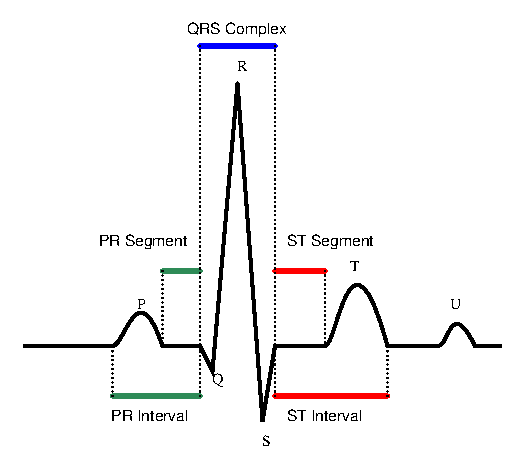
\includegraphics[width=4 cm,height=2.5 cm,angle=360]{Figures/01ECGSignal.ps}
%				\end{figure}
%				\scriptsize{ \color{blue}{Electrocardiogram(ECG) signal}} \\
%			\end{center}
%		\column{2.5 in}
%			\begin{center}
%				\begin{figure}
%					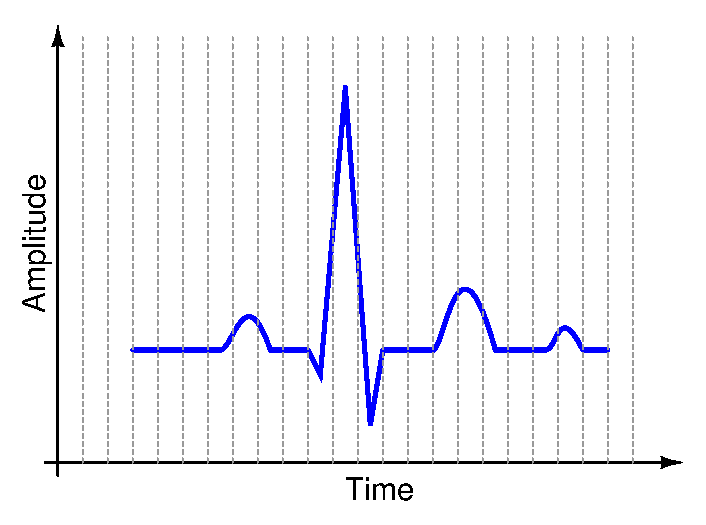
\includegraphics[width=4.5 cm,height=2.5 cm,angle=360]{Figures/02ECGSignal.ps}
%				\end{figure}
%				\scriptsize{ \color{blue}{Nyquist sampling for ECG signal}}
%			\end{center}
%			\begin{center}
%				\begin{figure}
%					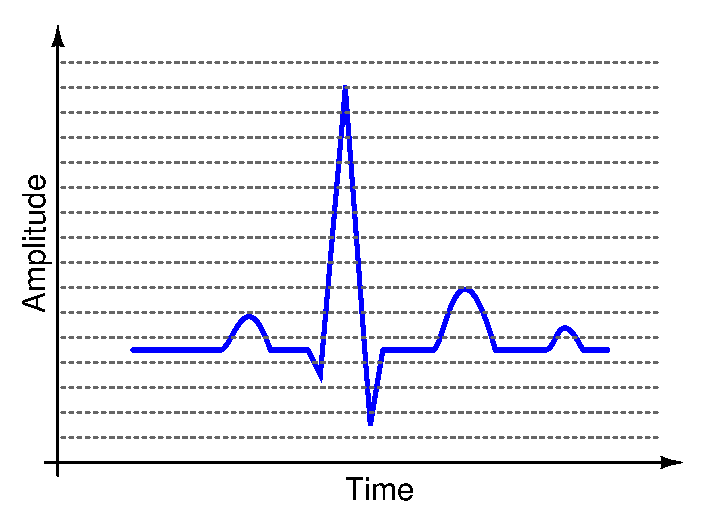
\includegraphics[width=4.5 cm,height=2.5 cm,angle=360]{Figures/03ECGSignal.ps}
%				\end{figure}
%				\scriptsize{ \color{blue}{Level cross sampling for ECG signal}}
%			\end{center}
%		\end{columns}
%	\end{center}
%\end{frame}
%%---------------------------------------------------------------------------------------------------------------------------%
%%-----------------------------------------Theory of Level Crossing Sampling Scheme------------------------------------------%
%%---------------------------------------------------------------------------------------------------------------------------%
%\section{Theory of level cross sampling}
%\subsection*{Level cross sampling scheme}
%\begin{frame}
%	\frametitle{Level crossing sampling scheme} \footnotesize
%	\begin{itemize}
%		\item{The principle of level crossing sampling is the dual of Nyquist sampling.}		
%		\item{A sample is taken only when $V_{in}$ crosses one of quantization levels.}\\
%		\item{It leads to reduction in no of digital samples and activity of the circuit.}\\
%		\item{Level cross sampling scheme simplifies design of Asynchronous ADCs.}\\			
%        \end{itemize}
%	\begin{center}
%		\begin{figure}
%			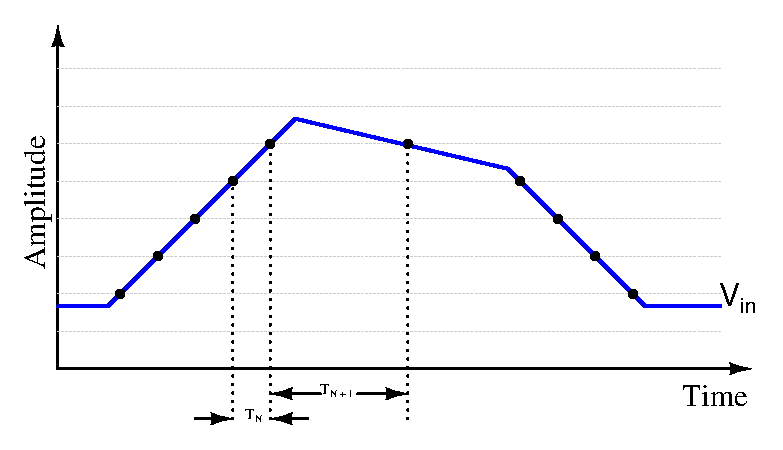
\includegraphics[width=7 cm,height=3.5 cm,angle=360]{Figures/04LCSScheme.ps}\\
%		\end{figure}
%		\scriptsize{ \color{blue}{Level Cross Sampling Scheme}}
%	\end{center}
%\end{frame}
%%---------------------------------------------------------------------------------------------------------------------------% 
%%---------------------------------------------------------------------------------------------------------------------------%
%\subsection*{Level cross sampling vs Nyquist sampling}
%\begin{frame}
%	\frametitle{Level cross vs Nyquist sampling} \scriptsize
%	\footnotesize{Difference between Nyquist sampling \& Level cross sampling schemes}
%	\begin{center}
%		\begin{tabular}{c|c|c|}
%			\cline {2-3} %\hline
%    			 &\footnotesize{\color{blue}{Nyquist sampling}} & \footnotesize{\color{blue}{Level cross sampling}} \\ \hline
%			\multicolumn {1}{|c|} {\footnotesize{\color{blue}{Conversion trigger}}} &  \scriptsize {Clock} & \scriptsize {Level crossing} \\ \hline
%			\multicolumn {1}{|c|} {\footnotesize{\color{blue}{Amplitude}}} & \scriptsize {Quantized} & \scriptsize {Exact value} \\ \hline
%			\multicolumn {1}{|c|} {\footnotesize{\color{blue}{Time}}} & \scriptsize {Exact value} & \scriptsize {Quantized} \\ \hline
%			\multicolumn {1}{|c|} {\footnotesize{\color{blue}{SNR dependency}}} & \scriptsize {Number of bits} & \scriptsize {Timer period} \\ \hline
%			\multicolumn {1}{|c|} {\footnotesize{\color{blue}{Converter output}}} & \scriptsize {Amplitude} & \scriptsize {Amplitude \& Time} \\ \hline
%		\end{tabular} \\
%	\end{center}
%	\vspace{5 mm}
%	\footnotesize{Advantages of level cross sampling over Nyquist sampling}
%	\begin{center}
%		\begin{itemize} \scriptsize
%			\item{Reduction in number of samples from ADC} \\
%			\item{Reduction in activity of the ADC circuit} \\
%		\end{itemize}
%	\end{center}
%\end{frame}
%%---------------------------------------------------------------------------------------------------------------------------%
%%---------------------------------------------------------------------------------------------------------------------------%
%\subsection*{Level crossing asynchronous ADC architecture}
%\begin{frame}
%	\frametitle{Level crossing asynchronous ADC} \footnotesize
%	\begin{center}
%		\begin{figure}
%			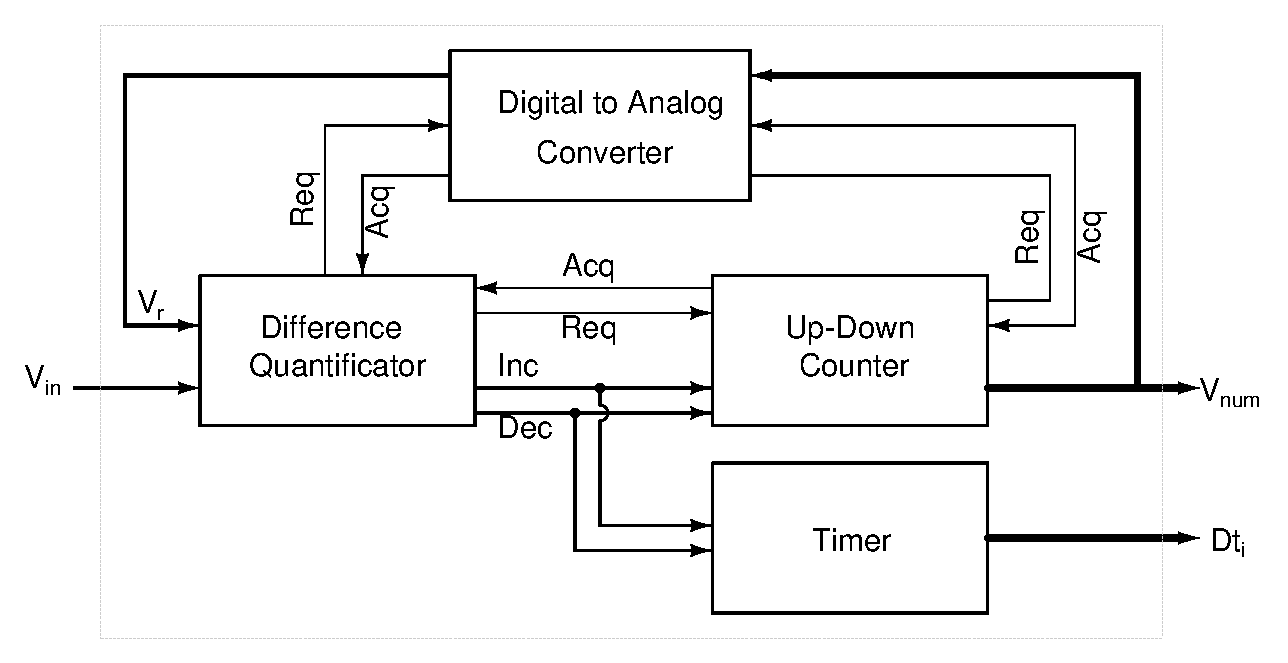
\includegraphics[width=10 cm,height=5 cm,angle=360]{Figures/05ADCAsync.ps}\\
%		\end{figure}
%		\scriptsize{ \color{blue}{Block diagram of the level crossing asynchronous ADC}}
%	\end{center}
%\let\thefootnote\relax\footnotetext[\value{footnote}]{\tiny{\color{blue}E. Allier et. al "A 120nm low power asynchronous ADC" 2005. }}
%\end{frame}
%%---------------------------------------------------------------------------------------------------------------------------%
%\begin{frame}
%	\frametitle{Drawbacks of level crossing asynchronous ADC} \footnotesize
%	\begin{center}
%		\begin{figure}
%			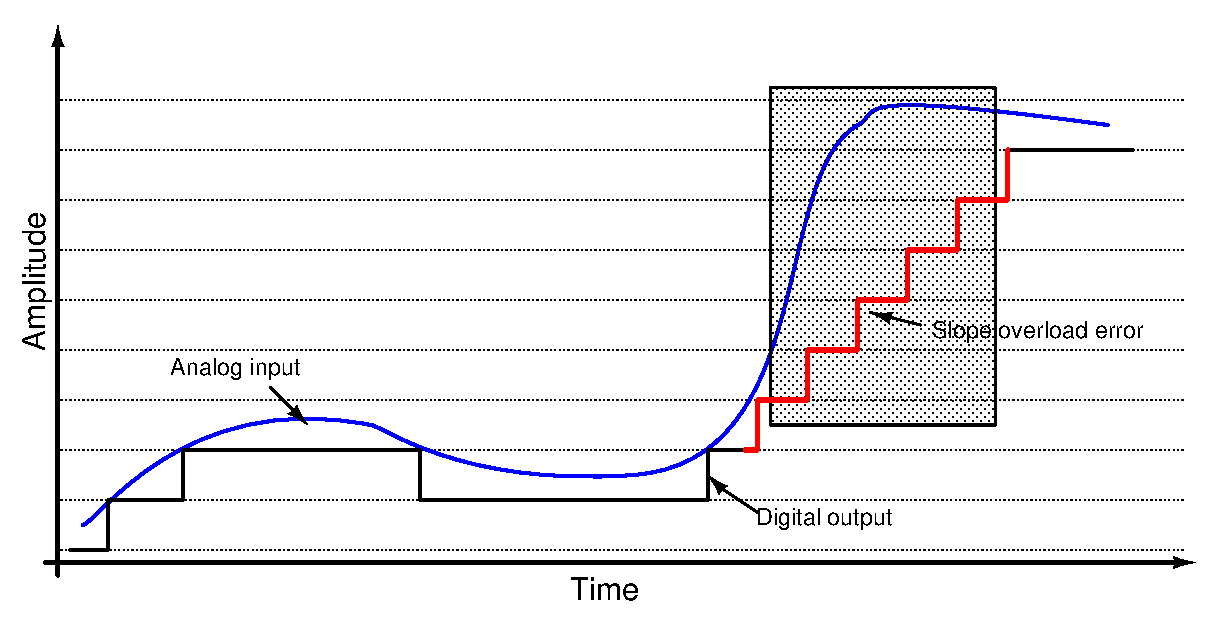
\includegraphics[width=10 cm,height=5 cm,angle=360]{Figures/06LCSPSpeed.ps}\\
%		\end{figure}
%		\scriptsize{ \color{blue}{Waveform showing slope overload error in level crossing ADC}}
%	\end{center}
%\end{frame}
%%---------------------------------------------------------------------------------------------------------------------------%
%\begin{frame}
%	\frametitle{Signal dependent variable resolution ADC} \footnotesize
%	\begin{center}
%		\begin{figure}
%			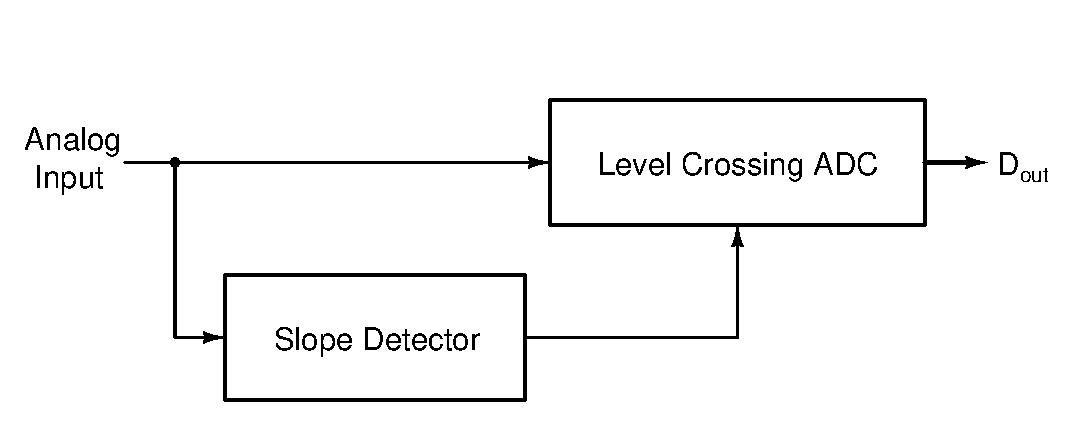
\includegraphics[width=10 cm,height=4 cm,angle=360]{Figures/07ADCsdvr.ps}\\
%		\end{figure}
%		\scriptsize{ \color{blue}{Block diagram of the signal dependent variable resolution ADC}}
%	\end{center}
%\let\thefootnote\relax\footnotetext[\value{footnote}]{\tiny{\color{blue}M. Kurchuk et. al "Signal-dependent variable-resolution quantization for continuous-time DSP" 2009. }}
%\end{frame}
%%---------------------------------------------------------------------------------------------------------------------------%
%\begin{frame}
%	\frametitle{Adaptive asynchronous ADC} \footnotesize
%	\begin{center}
%		\begin{figure}
%			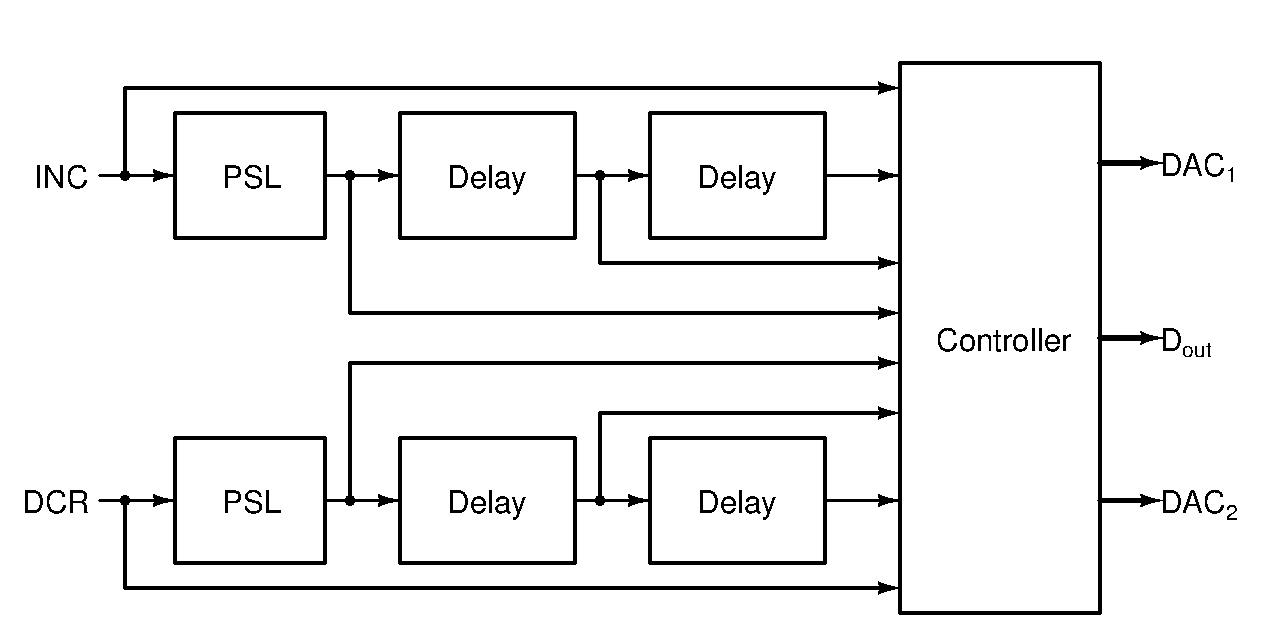
\includegraphics[width=10 cm,height=5 cm,angle=360]{Figures/08ADCaa.ps}\\
%		\end{figure}
%		\scriptsize{ \color{blue}{Block diagram of the adaptive asynchronous ADC}}
%	\end{center}
%\let\thefootnote\relax\footnotetext[\value{footnote}]{\tiny{\color{blue}R. Agarwal et. al "Adaptive asynchronous A to D conversion for compressed biomedical sensing" 2009. }}
%\end{frame}
%%---------------------------------------------------------------------------------------------------------------------------%
%%----------------------------------------------------Proposed ADC Architectures---------------------------------------------%
%%---------------------------------------------------------------------------------------------------------------------------%
%\section{Proposed ADC architectures}
%\subsection*{Controller for high activity ratio signals}
%\begin{frame}
%	\frametitle{Controller operation for high activity ratio signals } \footnotesize
%	\begin{center}
%		\begin{columns}[c]
%		\column{2.5 in}
%			\begin{center}
%				\begin{figure}
%					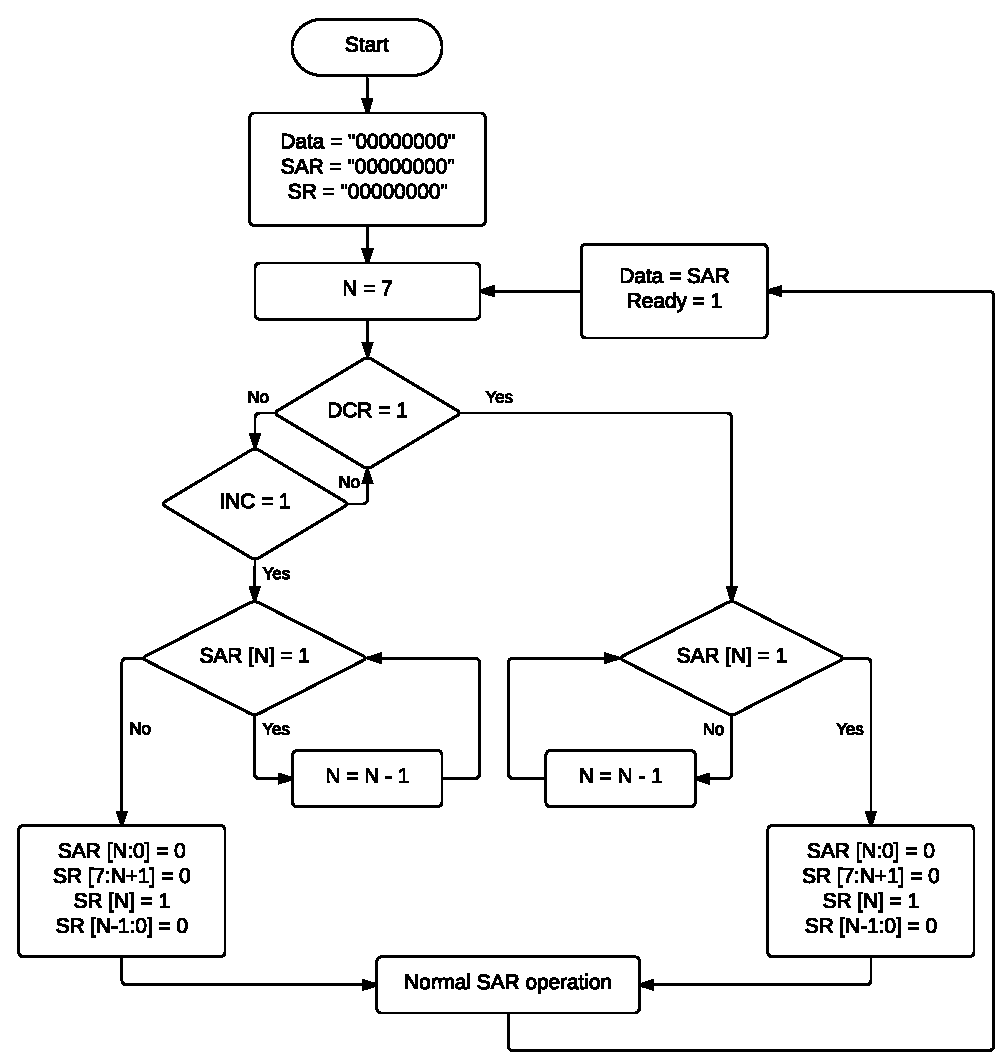
\includegraphics[width=6 cm,height=6 cm,angle=360]{Figures/10HARsig.ps}
%				\end{figure}
%				\scriptsize{ \color{blue}{Controller for high activity ratio signals }}
%			\end{center}

%		\column{2.5 in}
%			\begin{center}
%				\begin{figure}
%					\includegraphics[width=5.5 cm]{Figures/12HARmatlab.eps}
%				\end{figure}
%				\scriptsize{ \color{blue}{Number of clock cycles needed for conversion}}
%			\end{center}
%		\end{columns}
%	\end{center}
%\end{frame}
%%---------------------------------------------------------------------------------------------------------------------------%
%\begin{frame}
%	\frametitle{Controller operation for high activity ratio signals } \footnotesize
%	\begin{center}

%	\end{center}
%\end{frame}
%%---------------------------------------------------------------------------------------------------------------------------%
%\begin{frame}
%	\frametitle{Controller operation for high activity ratio signals } \footnotesize
%	\begin{center}

%	\end{center}
%\end{frame}
%%---------------------------------------------------------------------------------------------------------------------------%
%%---------------------------------------------------------------------------------------------------------------------------%
%\subsection*{Controller for low activity ratio signals}
%\begin{frame}
%	\frametitle{Controller operation for low activity ratio signals} \footnotesize
%	\begin{center}
%		\begin{columns}[c]
%		\column{2.5 in}
%			\begin{center}
%				\begin{figure}
%					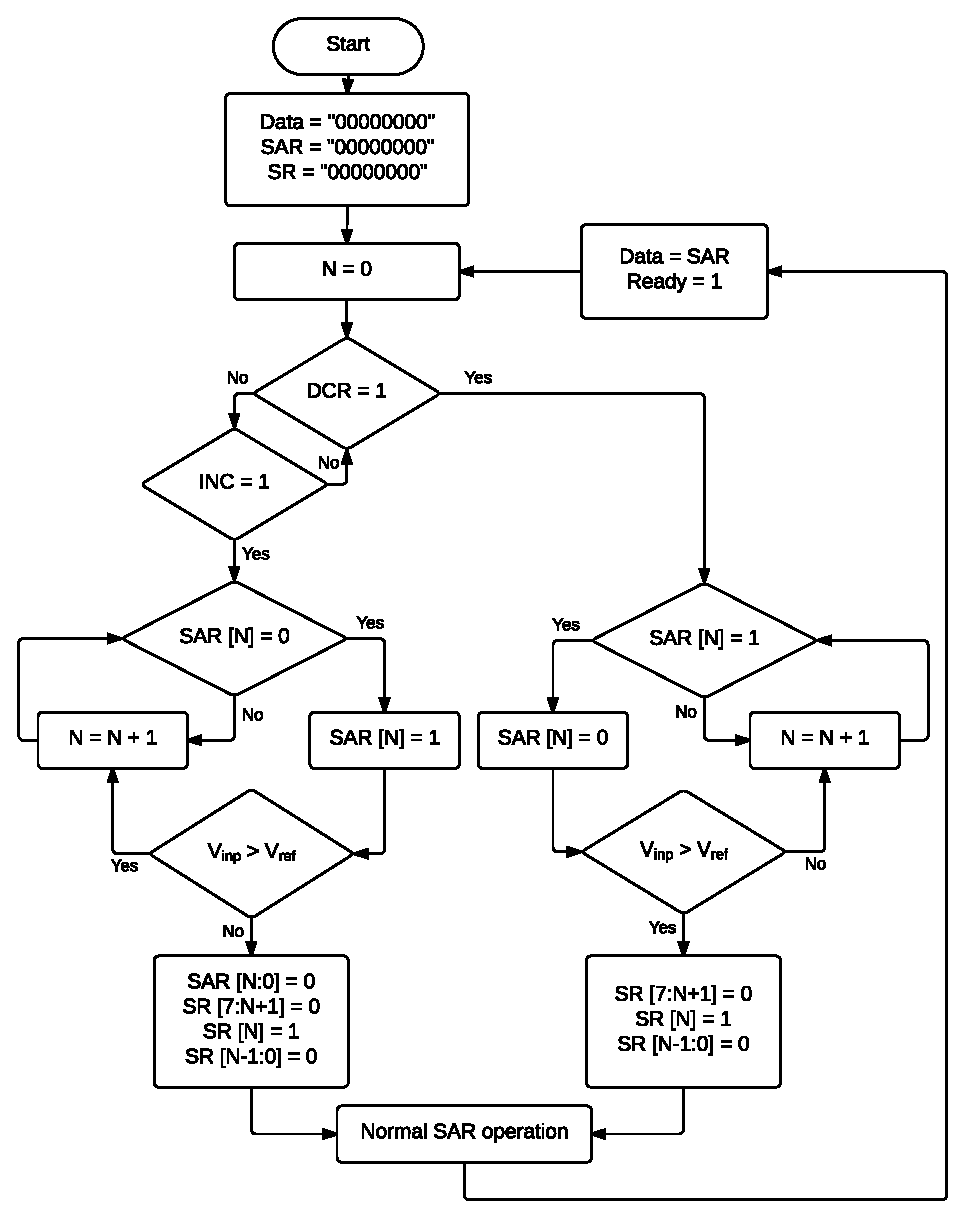
\includegraphics[width=5.5 cm,height=6 cm,angle=360]{Figures/11LARsig.ps}
%				\end{figure}
%				\scriptsize{ \color{blue}{Controller for low activity ratio signals }}
%			\end{center}

%		\column{2.5 in}
%			\begin{center}
%				\begin{figure}
%					\includegraphics[width=5.5 cm]{Figures/14LARmatlab.eps}
%				\end{figure}
%				\scriptsize{ \color{blue}{Number of clock cycles needed for conversion}}
%			\end{center}
%		\end{columns}
%	\end{center}
%\end{frame}
%%---------------------------------------------------------------------------------------------------------------------------%
%\begin{frame}
%	\frametitle{Controller operation for low activity ratio signals} \footnotesize
%	\begin{center}

%	\end{center}
%\end{frame}
%%---------------------------------------------------------------------------------------------------------------------------%
%\begin{frame}
%	\frametitle{Controller operation for low activity ratio signals} \footnotesize
%	\begin{center}

%	\end{center}
%\end{frame}
%%---------------------------------------------------------------------------------------------------------------------------%
%%---------------------------------------------------------------------------------------------------------------------------%
%\subsection*{Controller for modified Sucssive Aproximation}
%\begin{frame}
%	\frametitle{Controller operation for modified Sucssive Aproximation } \footnotesize
%	\begin{center}
%		\begin{columns}[c]
%		\column{2.5 in}
%			\begin{center}
%				\begin{figure}
%					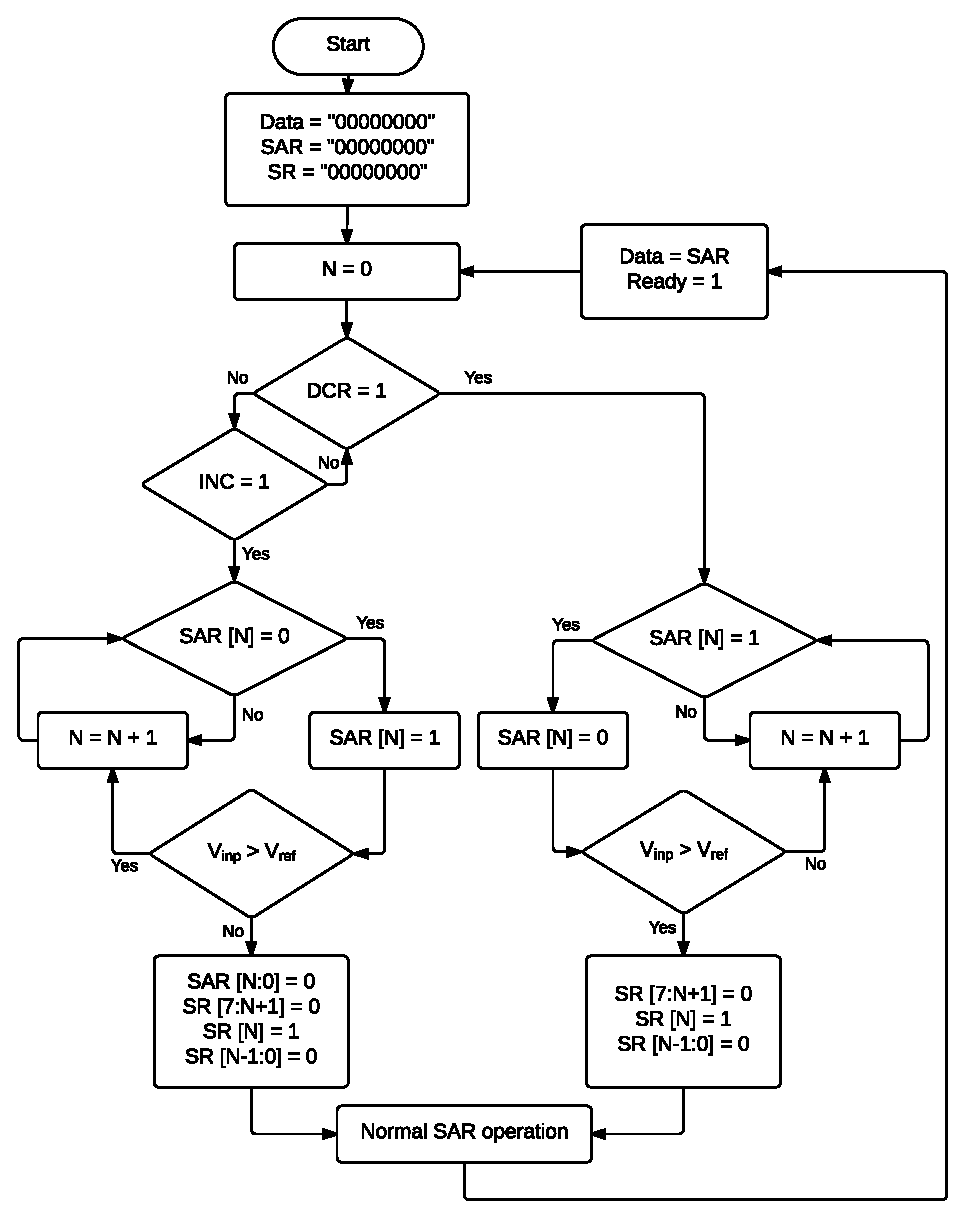
\includegraphics[width=5.5 cm,height=6 cm,angle=360]{Figures/11LARsig.ps}
%				\end{figure}
%				\scriptsize{ \color{blue}{Controller for modified Sucssive Aproximation }}
%			\end{center}

%		\column{2.5 in}
%			\begin{center}
%				\begin{figure}
%					\includegraphics[width=5.5 cm]{Figures/14LARmatlab.eps}
%				\end{figure}
%				\scriptsize{ \color{blue}{Number of clock cycles needed for conversion}}
%			\end{center}
%		\end{columns}
%	\end{center}
%\end{frame}
%%---------------------------------------------------------------------------------------------------------------------------%
%\begin{frame}
%	\frametitle{Controller operation for modified Sucssive Aproximation} \footnotesize
%	\begin{center}

%	\end{center}
%\end{frame}
%%---------------------------------------------------------------------------------------------------------------------------%
%\begin{frame}
%	\frametitle{Controller operation for modified Sucssive Aproximation} \footnotesize
%	\begin{center}

%	\end{center}
%\end{frame}
%---------------------------------------------------------------------------------------------------------------------------% 
%----------------------------------------------------Conclusion and Future Work---------------------------------------------%
%---------------------------------------------------------------------------------------------------------------------------%
\section{Simulation results \& Future work}
\subsection*{Simulation results}
\begin{frame}
	\frametitle{Building Blocks for proposed ADC} \footnotesize
	\begin{itemize} 
		\item{ ADC specifications}
			\begin{itemize} \scriptsize
				\item{ Technology - UMC 180nm } \\
				\item{ Power supply - 1.8 V } \\
				\item{ Resolution - 8-bit  } \\
				\item{ Peak to peak analog input voltage - 1 V (0.4 to 1.4)} \\
				\item{ Maximum analog input frequency - 20K Hz } \\
			\end{itemize}
		\item{ Analog Blocks }\\
			\begin{itemize} \scriptsize
				\item{ Clocked Comparator } \\
				\item{ Track \& Hold } \\
				\item{ Non Overlapping Clock Generator } \\
				\item{ Driver Network } \\
				\item{ Binary Weighted Capacitor Array  } \\
			\end{itemize}
	\end{itemize}
\end{frame}
%---------------------------------------------------------------------------------------------------------------------------%
\begin{frame}
	\frametitle{Comparision between architectures} \footnotesize
	\begin{center}

	\end{center}
\end{frame}
%---------------------------------------------------------------------------------------------------------------------------%
%---------------------------------------------------------------------------------------------------------------------------% 
\subsection*{Future work}
\begin{frame}
	\frametitle{Future work} \footnotesize
	\begin{itemize} 
		\item{ Future Work}
			\begin{itemize} \scriptsize
			\item{ Complete the connections between individual modules. }\\
			\item{ Complete the layout of capacitor array \& Switching network. } \\ 
			\item{ Complete the place \& route of controller blocks. }
			\item{ Send both designs for tapeouts in August.} \\
			\item{ Modify the proposed architecture for repetitive signals.} \\
			\end{itemize}
		\item{ Problems encountered when implementing design}
			\begin{itemize} \scriptsize
			\item{ Applying Timing constraints for multiple clock domains. } \\
			\item{ Problem with the capacitor layout because of multiplier. } \\ 
			\item{ Problem with the capacitor layout because of parasitics. } \\ 
			\end{itemize}
		\item{ Prsently working on Connecting digital controller circuit with analog blocks.}
	\end{itemize}
\end{frame}
%---------------------------------------------------------------------------------------------------------------------------%
%-------------------------------------------------------References----------------------------------------------------------%
%---------------------------------------------------------------------------------------------------------------------------%
\subsection*{References}
\begin{frame}
	\frametitle{References}
	\begin{thebibliography}{12}
	\tiny { 	\bibitem{1P} E. Allier, J. Goulier, G. Sicard, A. Dezzani, E. Andre and M. Renaudin, "A 120nm low power asynchronous ADC,"
 				\emph {International Symposium on Low Power Electronics and Design}, 2005.

				\bibitem{7P} E. Allier, G. Sicard, L. Fesquet and M. Renaudin, "Asynchronous level crossing analog to digital converters," 
				\emph {Elsevier Journal of the International Measurement Confederation}, 2005.

				\bibitem{4P} E. Allier, G. Sicard, L. Fesquet, M. Renaudin,  "A New Class of Asynchronous A/D Converters Based on Time Quantization," 
				\emph {International Symposium on Asynchronous Circuits and Systems}, 2003.

				\bibitem{3P} R. Agarwal, M. Trakimas and S. Sonkusale, "Adaptive asynchronous analog to digital conversion for compressed biomedical sensing,"
				\emph {IEEE Conference on Biomedical Circuits and Systems}, 2009.

				\bibitem{8P} A. Fayed and M. Ismail, "A High Speed, Low Voltage CMOS Offset Comparator," 
				\emph {Analog Integrated Circuits and Signal Processing}, 2003.

				\bibitem{9P} Daegyu Lee, Jincheol Yoo, Kyusun Choi and J. Ghaznavi, "Fat tree encoder design for ultra-high speed flash A/D converters,"
				\emph { Midwest Symposium on Circuits and Systems}, 2002.

				\bibitem{2P} F. Akopyan, R. Manohar, and A. B. Apsel, "A level-crossing flash asynchronous analog-to-digital converter," 
				\emph {International Symposium on Asynchronous Circuits and Systems}, 2006. }
	\end{thebibliography}
\end{frame}
%---------------------------------------------------------------------------------------------------------------------------%
\begin{frame}
	\frametitle{References}
	\begin{thebibliography}{12}
	\tiny { 	\bibitem{1P} E. Allier, J. Goulier, G. Sicard, A. Dezzani, E. Andre and M. Renaudin, "A 120nm low power asynchronous ADC,"
 				\emph {International Symposium on Low Power Electronics and Design}, 2005.

				\bibitem{7P} E. Allier, G. Sicard, L. Fesquet and M. Renaudin, "Asynchronous level crossing analog to digital converters," 
				\emph {Elsevier Journal of the International Measurement Confederation}, 2005.

				\bibitem{4P} E. Allier, G. Sicard, L. Fesquet, M. Renaudin,  "A New Class of Asynchronous A/D Converters Based on Time Quantization," 
				\emph {International Symposium on Asynchronous Circuits and Systems}, 2003.

				\bibitem{3P} R. Agarwal, M. Trakimas and S. Sonkusale, "Adaptive asynchronous analog to digital conversion for compressed biomedical sensing,"
				\emph {IEEE Conference on Biomedical Circuits and Systems}, 2009.

				\bibitem{8P} A. Fayed and M. Ismail, "A High Speed, Low Voltage CMOS Offset Comparator," 
				\emph {Analog Integrated Circuits and Signal Processing}, 2003.

				\bibitem{9P} Daegyu Lee, Jincheol Yoo, Kyusun Choi and J. Ghaznavi, "Fat tree encoder design for ultra-high speed flash A/D converters,"
				\emph { Midwest Symposium on Circuits and Systems}, 2002.

				\bibitem{2P} F. Akopyan, R. Manohar, and A. B. Apsel, "A level-crossing flash asynchronous analog-to-digital converter," 
				\emph {International Symposium on Asynchronous Circuits and Systems}, 2006. }
	\end{thebibliography}
\end{frame}
%---------------------------------------------------------------------------------------------------------------------------%
%-----------------------------------------------------End of Presentation---------------------------------------------------%
%---------------------------------------------------------------------------------------------------------------------------%

\end{document}

